\begin{code}[hide]
module slides.Tsinghua-PL-seminar.sections.newcore where

open import Data.Nat using (ℕ)
open import Data.Product using (Σ ; _×_ ; _,_)
open import Level using (0ℓ)
open import Relation.Binary using (Rel)
open import Relation.Nullary using (¬_)
open import Relation.Binary.PropositionalEquality using (_≢_)
open import Algebra.Bundles using (Monoid)

open import Notations using (₁₊ ; ₂₊)
open import Word.Base using (Word ; WRel ; [_]ʷ ; ε ; _•_ ; wmap)

postulate
  proof-elided : ∀ {ℓ} {A : Set ℓ} → A
  Gate : ℕ → Set
  X : Set

private variable
  n : ℕ
\end{code}
%% Part 6a — what happened after the submission; the core library.
\NewPart
\section{New since the paper}

\begin{frame}{What happened after the submission \New}
\begin{columns}[c]
\begin{column}{0.58\textwidth}
\centering
\begin{tikzpicture}[x=5.3mm,y=6.6mm,>={Stealth[length=1.6mm]},
  lb/.style={font=\scriptsize,anchor=west,align=left}]
  % trunk
  \draw[thick,paperC] (0,0) -- (3,0);
  \node[cm=paperC,label={[font=\scriptsize,align=center]below:tag\\[-2pt]\texttt{popl-revision1}}] at (0,0) {};
  \node[font=\tiny,gray] at (0,0.45) {Jul};
  \draw[thick,accent] (3,0) -- (6,0);
  \node[cm=accent,label={[font=\scriptsize]below:\texttt{main}}] at (6,0) {};
  \node[font=\tiny,gray] at (6,0.45) {Sep 2};
  % branches
  \draw[thick,newC] (6,0) .. controls (7,0) and (7,2.4) .. (9.5,2.4) node[cm=newC] {} node[lb,right=2pt]{\texttt{popl}\\[-1pt]path sums};
  \draw[thick,newC] (6,0) .. controls (7,0) and (7,0.8) .. (9.5,0.8) node[cm=newC] {} node[lb,right=2pt]{\texttt{v-office}\\[-1pt]unitary groups};
  \draw[thick,newC] (6,0) .. controls (7,0) and (7,-0.8) .. (9.5,-0.8) node[cm=newC] {} node[lb,right=2pt]{\texttt{qupit}\\[-1pt]minimality, CNOT-dihedral};
  \draw[thick,newC] (6,0) .. controls (7,0) and (7,-2.4) .. (9.5,-2.4) node[cm=newC] {} node[lb,right=2pt]{\texttt{v-office-Cli-CH}\\[-1pt]Real-Clifford+$CH$};
  \node[font=\scriptsize,align=center,accent] at (4.5,-1.6) {qupit Clifford,\\$Sp(2n,\mathbb{Z}_p)$,\\exact Clifford};
  \draw[->,gray] (4.5,-1.0) -- (4.5,-0.15);
  \node[font=\tiny,gray] at (9.5,3.1) {late Sep -- Oct 2026};
\end{tikzpicture}
\end{column}
\begin{column}{0.40\textwidth}
\centering
\begin{tikzpicture}
\begin{axis}[xbar, width=5.4cm, height=5.2cm, xmin=0, xmax=230,
  symbolic y coords={v-office-Cli-CH,qupit,v-office,popl,main,tag},
  ytick=data, y tick label style={font=\scriptsize\ttfamily},
  x tick label style={font=\scriptsize}, xlabel={\scriptsize thousand lines of Agda},
  nodes near coords, nodes near coords style={font=\tiny},
  bar width=7pt, enlarge y limits=0.12, axis lines*=left]
\addplot[fill=paperC!70,draw=paperC] coordinates {(22.2,tag)};
\addplot[fill=newC!60,draw=newC] coordinates
  {(112.8,main) (193.9,popl) (155.2,v-office) (139.9,qupit) (187.1,v-office-Cli-CH)};
\end{axis}
\end{tikzpicture}

{\scriptsize \texttt{*.agda} outside \texttt{paper/}; 74 files at the tag,
634 on \texttt{v-office-Cli-CH}}
\end{column}
\end{columns}
\end{frame}

\begin{frame}{Research papers formalized since the submission \New}
\centering\scriptsize
\renewcommand{\arraystretch}{1.18}
\begin{tabular}{@{}p{4.0cm}p{2.7cm}p{2.6cm}p{4.0cm}@{}}
\toprule
paper formalized & gate set / group & semantics & status\\
\midrule
Bian, Li, Ross, van de Wetering, Zhao (QPL'26): qupit Clifford, all odd primes
  & $H,S,CZ$; $\text{Pauli}\rtimes Sp(2n,\mathbb{Z}_p)$ & symplectic maps, Pauli action & \textbf{complete}, every $n$, every odd prime $p$\\
Selinger (LMCS 2015): $n$-qubit Clifford & $\omega,H,S,CZ$ & $Sp(2n,2)$ + phases & \textbf{complete} (modulo scalars; scalars as extension)\\
Bian--Selinger (QPL'21): $U_n(\mathbb{Z}[\frac12,i])$ & two-level $X,K,i$ & \alert{matrices} over $\mathbb{Z}[\frac12,i]$ & \textbf{complete}, every $n$\\
Greylyn (2014); Bian--Selinger (QPL'22): 2-qubit Clifford+$T$ & $\omega,H_i,S_i,T_i,CZ$ & \alert{matrices} over $\mathbb{Z}[\frac1{\sqrt2},i]$ & \textbf{complete} ($n\le4$; faithful into $U_4$)\\
Bian--Selinger (QPL'23): 3-qubit Clifford+$CS$ & $S_i, CS, K_i, i$ & matrices over $\mathbb{Z}[\frac12,i]$ & in progress (steps 1 and 4 of the R--S chain)\\
Clément (2026): Real-Clifford+$CH$ & $H,Z,CZ,CH$ & \alert{matrices} over $\mathbb{Z}[\sqrt2]$ & sound; complete on $\le1$ qubit; $\ge2$ modulo Thm 4.4 (imported by the paper too) + Lemma 8.8 at 3--4 qubits\\
Amy--Chen--Ross (QPL'17): CNOT-dihedral & $\omega,X,T,CNOT$ & phase polynomials & sound; complete on 1 qubit; $n$ modulo imported lemmas\\
Amy (QPL'18): path sums & $H,S,CZ$ / $H,CNOT,R_k$ & exact sums over $\mathbb{Z}[\zeta]$ & Clifford equivalence in \alert{polynomial cost}\\
\bottomrule
\end{tabular}

\vspace{4pt}
{\scriptsize plus, in the core: 0-ary gates (scalars), independence of axioms, central and
factor-set extensions, generic circuit coset towers}
\end{frame}

\begin{frame}{Scalars: 0-ary gates, and a rule that became a theorem \New}
\begin{columns}[c]
\begin{column}{0.55\textwidth}
\small Global phases ($\omega$, $\zeta$, \ldots) live on no wire, at every width:
\begin{code}
data Gen : ℕ → Set where
  gate₀ : Gate 0 → Gen n
  gate₁ : Gate 1 → Gen (₁₊ n)
  gate₂ : Gate 2 → Gen (₂₊ n)
  _↥   : Gen n → Gen (₁₊ n)
\end{code}
\begin{code}[hide]
Circuit : ℕ → Set
Circuit n = Word (Gen n)
CRel : ℕ → Set₁
CRel n = Rel (Circuit n) 0ℓ
_↑ : Circuit n → Circuit (₁₊ n)
_↑ = wmap _↥
infix 4 _SRel,_===_ _VRel,_===_ _≈_
postulate
  _SRel,_===_ : (n : ℕ) → WRel (Gen n)
  _≈_ : Circuit n → Circuit n → Set
private variable
  w v : Circuit n
\end{code}
\vspace{-6pt}
\small Four structural rules now (\Branch{qupit}, \texttt{Circuit/Base.agda}):
\begin{code}
data _VRel,_===_ : (n : ℕ) → CRel n where
  srel  : n SRel, w === v → n VRel, w === v
  cong↑ : n VRel, w === v → (₁₊ n) VRel, w ↑ === v ↑
  comm₁ : (h : Gate 1) (g : Gen n) → (₁₊ n) VRel,
          [ g ↥ ]ʷ • [ gate₁ h ]ʷ === [ gate₁ h ]ʷ • [ g ↥ ]ʷ
  comm₂ : (h : Gate 2) (g : Gen n) → (₂₊ n) VRel,
          [ g ↥ ↥ ]ʷ • [ gate₂ h ]ʷ === [ gate₂ h ]ʷ • [ g ↥ ↥ ]ʷ
  ω↑=ω : (ω : Gate 0) → (₁₊ n) VRel, [ gate₀ ω ]ʷ ↑ === [ gate₀ ω ]ʷ
\end{code}
\end{column}
\begin{column}{0.42\textwidth}
\renewcommand{\AgdaCodeStyle}{\scriptsize}
\small There is \alert{no} \aid{comm₀} rule: centrality of a scalar is a
\emph{theorem}, from the other rules plus one hypothesis --- that scalars
commute with each other:
\begin{code}
module Central-Scalars
  (scalars-comm : ∀ {n} (h h' : Gate 0) →
     [ gate₀ {n} h' ]ʷ • [ gate₀ h ]ʷ
       ≈ [ gate₀ h ]ʷ • [ gate₀ h' ]ʷ)
  where
  comm₀ : ∀ (h : Gate 0) (g : Gen n) →
          [ g ]ʷ • [ gate₀ h ]ʷ ≈ [ gate₀ h ]ʷ • [ g ]ʷ
\end{code}
\begin{code}[hide]
  comm₀ = proof-elided
\end{code}
{\scriptsize (the \aid{let open PB …} of the source elided)}

\vspace{4pt}
\begin{tikzpicture}[x=5mm,y=5mm,line width=0.7pt]
  \foreach \y in {0,1,2} \draw (0,\y) -- (4,\y);
  \node[draw,fill=softnew,circle,inner sep=1pt,font=\scriptsize] at (1,2.9) {$\omega$};
  \node[draw,fill=white,font=\scriptsize,minimum size=4mm,inner sep=0pt] at (2.6,0) {$h$};
  \node at (5,1) {$\approx$};
  \foreach \y in {0,1,2} \draw (6,\y) -- (10,\y);
  \node[draw,fill=softnew,circle,inner sep=1pt,font=\scriptsize] at (8.6,2.9) {$\omega$};
  \node[draw,fill=white,font=\scriptsize,minimum size=4mm,inner sep=0pt] at (7,0) {$h$};
\end{tikzpicture}
\end{column}
\end{columns}
\end{frame}

\begin{frame}{Minimality: when is a rule \emph{not} derivable from the others? \New}
\begin{code}[hide]
module Indep where
  infixl 8 _∣_
  postulate
    Derivable : ∀ {Γ : WRel X} {P : Set} → Set
    ⟦_⟧ : Word X → X
    _≈ᴹ_ : X → X → Set
\end{code}
\begin{columns}[c]
\begin{column}{0.56\textwidth}
\small \texttt{Presentation/Independence.agda} (\Branch{qupit}): select some
axiom \emph{instances}; is another one derivable from them?
\begin{code}
  Select : WRel X → Set₁
  Select Γ = ∀ {w v} → Γ w v → Set

  _∣_ : (Γ : WRel X) → Select Γ → WRel X
  (Γ ∣ P) w v = Σ (Γ w v) P
\end{code}
\begin{code}[hide]
  postulate
    Independent : ∀ (Γ : WRel X) (P : Select Γ) {w v} → Γ w v → Set
  module Model (Γ : WRel X) (P : Select Γ) (mon : Monoid 0ℓ 0ℓ) (⟦_⟧₀ : X → Monoid.Carrier mon) where
   module Sound where
\end{code}
\par\medskip
\small A \alert{model}: a monoid where the selected axioms hold. It
separates the instance's two sides $\Rightarrow$ the instance is independent:
\begin{code}
    independent : (a : Γ w v) → ¬ (⟦ w ⟧ ≈ᴹ ⟦ v ⟧) → Independent Γ P a
\end{code}
\begin{code}[hide]
    independent = proof-elided
\end{code}
{\scriptsize (\aid{\_≈ᴹ\_} is the monoid's \aid{\_≈\_} in the source)}
\end{column}
\begin{column}{0.41\textwidth}
\centering
\begin{tikzpicture}[>={Stealth[length=1.8mm]}]
  \node[draw=accent,fill=soft,rounded corners=3pt,minimum width=40mm,minimum height=26mm] (R) at (0,0) {};
  \node[font=\scriptsize\bfseries,accent,anchor=north west] at (R.north west) {axiom instances of $\Gamma$};
  \foreach \x/\y in {-1.4/0.3,-0.8/-0.4,-0.2/0.2,0.4/-0.5,1.0/0.1,-1.1/-0.9,0.1/-1.0} \node[circle,fill=paperC,inner sep=1.4pt] at (\x,\y) {};
  \node[circle,fill=newC,inner sep=2pt,label={[font=\scriptsize,newC]right:$a$}] (a) at (1.25,-0.75) {};
  \draw[dashed,paperC,rounded corners] (-1.75,-1.2) rectangle (1.3,0.55);
  \node[font=\tiny,paperC] at (-0.3,0.7) {selected $P$};
  \node[draw=gray,fill=white,rounded corners=2pt,font=\scriptsize,align=center] (M) at (0,-2.4) {model $\mathcal{M}$: all of $P$ hold,\\ $\llbracket w\rrbracket\neq\llbracket v\rrbracket$ for $a : w = v$};
  \draw[->,thick,gray] (M) -- (0,-1.32);
\end{tikzpicture}

\vspace{6pt}
{\small soundness extends from axioms to the whole congruence of $\Gamma\mid P$
by \aid{StarInterp}: a separated instance is not derivable.}
\end{column}
\end{columns}
\end{frame}

\begin{frame}{The structural rules are mutually independent \New}
\begin{code}[hide]
data Rule : Set where
  cong↑ comm₁ comm₂ ω↑=ω : Rule
infix 4 _IndependentOf_
postulate
  _IndependentOf_ : ∀ {w v : Circuit n} → n VRel, w === v → Rule → Set
module Pure where
\end{code}
\begin{columns}[c]
\begin{column}{0.56\textwidth}
\renewcommand{\AgdaCodeStyle}{\scriptsize}
\small Over \emph{any} gate family, for the pure structural theory
(\texttt{Circuit/Independence.agda}), each rule fails in a model of the other three:
\begin{code}
  comm₁-independent : (h : Gate 1) →
                      comm₁ h (gate₁ {n} h) IndependentOf comm₁
  ω↑=ω-independent : (ω : Gate 0) → ω↑=ω {n} ω IndependentOf ω↑=ω
  cong↑-independent₁ : (h : Gate 1) →
                       cong↑ (comm₁ h (gate₁ {n} h)) IndependentOf cong↑
\end{code}
\begin{code}[hide]
  comm₁-independent = proof-elided
  ω↑=ω-independent = proof-elided
  cong↑-independent₁ = proof-elided
\end{code}
\small and the hypothesis of \aid{Central-Scalars} is \alert{needed}:
\begin{code}
  scalars-comm-needed : (ω ω' : Gate 0) → ω ≢ ω' →
    ¬ ([ gate₀ {n} ω' ]ʷ • [ gate₀ ω ]ʷ
         ≈ [ gate₀ ω ]ʷ • [ gate₀ ω' ]ʷ)
\end{code}
\begin{code}[hide]
  scalars-comm-needed = proof-elided
\end{code}
\end{column}
\begin{column}{0.41\textwidth}
\scriptsize
\renewcommand{\arraystretch}{1.15}
\begin{tabular}{@{}p{1.25cm}p{3.9cm}@{}}
\toprule
rule & model separating it\\
\midrule
\aid{ω↑=ω} & letter $\mapsto 2^{\mathit{depth}}$ in $(\mathbb{N},+)$; shift doubles\\
\aid{comm₁} & depths of 1-wire gates in \aid{List ℕ}; shift $=$ \aid{map suc}\\
\aid{comm₂} & the same, for 2-wire gates\\
\aid{cong↑} & read gates only at depth $\ge1$: no shift homomorphism\\
\aid{comm₀} & scalars in order, in \aid{List (Gate 0)}\\
\bottomrule
\end{tabular}

\vspace{6pt}
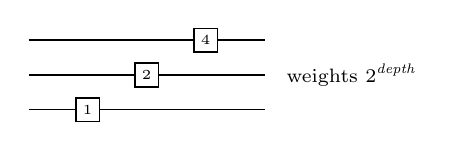
\begin{tikzpicture}[x=5mm,y=4.4mm,line width=0.6pt]
  \foreach \y in {0,1,2} \draw (0,\y) -- (6,\y);
  \node[draw,fill=white,font=\tiny,minimum size=3mm,inner sep=0pt] at (1.5,0) {$1$};
  \node[draw,fill=white,font=\tiny,minimum size=3mm,inner sep=0pt] at (3,1) {$2$};
  \node[draw,fill=white,font=\tiny,minimum size=3mm,inner sep=0pt] at (4.5,2) {$4$};
  \node[font=\scriptsize,anchor=west] at (6.3,1) {weights $2^{\mathit{depth}}$};
\end{tikzpicture}

\vspace{2pt}
{\scriptsize Scope today: the \emph{structural} rules. No gate-specific rule set is
shown minimal yet --- but several were \emph{reduced} by derivations
(next slides).}
\end{column}
\end{columns}
\end{frame}
